\begin{frame}{Experimental Results}{Success Rate}
     \small{Comparison with using the true I-state, we conducted experiments using 3
     environments, and 3 range spaces $\mathcal{R}_{disk}$, $\mathcal{R}_{rect}$,
     and  $\mathcal{R}_{drect}$. \\
     In each environment we collect the success rate of completing the navigation
     task. 
     \begin{enumerate}
     \item The number of landmarks $N$: between $5$ and $250$ in increments of $5$
     \item For each $N$, run the experiment 15 trials with different landmark
       distributions by assigning distinct random seeds
     \end{enumerate}
    }
    \only<1>{
        \centering
        \begin{figure}
          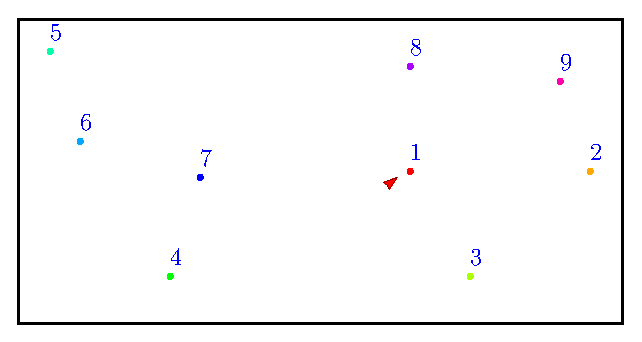
\includegraphics[width=0.65\textwidth]{figs/blank}
        \end{figure}
        Obstacle-free Environment
    }
    \only<2>{
        \centering
        \begin{figure}
          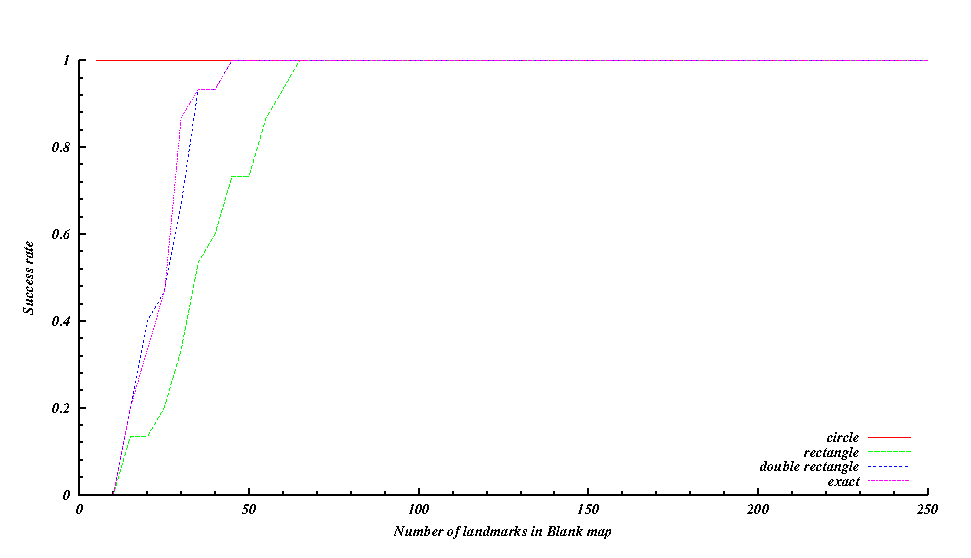
\includegraphics[width=0.67\textwidth]{Data/expnumblank}
        \end{figure}
        Success Rate for the Obstacle-free Environment
    }
    \only<3>{
        \centering
        \begin{figure}
            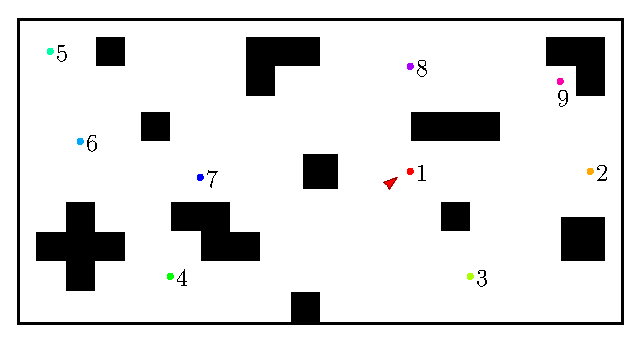
\includegraphics[width=0.65\textwidth]{figs/clutter}
        \end{figure}
        Obstacle-cluttered Environment
    }
    \only<4>{
        \centering
        \begin{figure}
            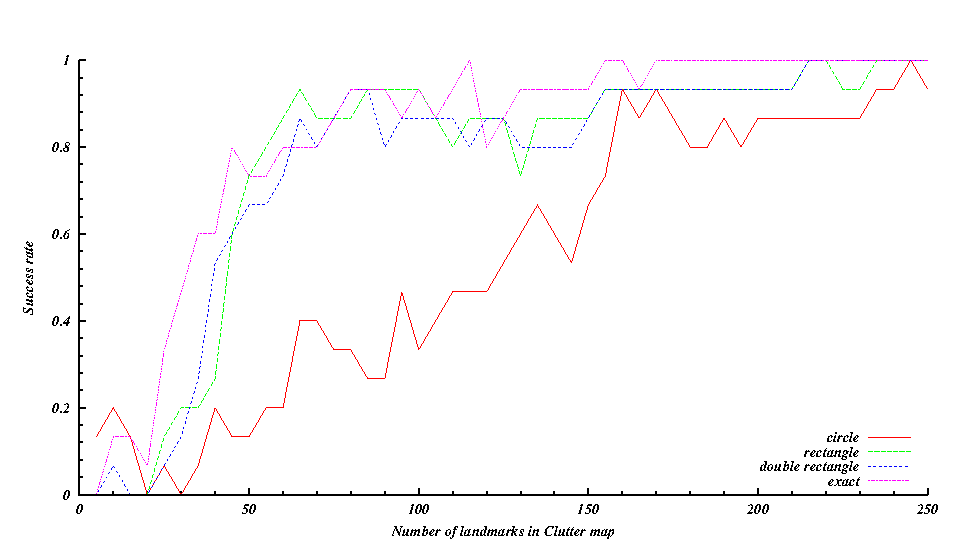
\includegraphics[width=0.67\textwidth]{Data/expnumclutter}
        \end{figure}
        Success Rate for the Obstacle-cluttered Environment
    }
    \only<5>{
        \centering
        \begin{figure}
            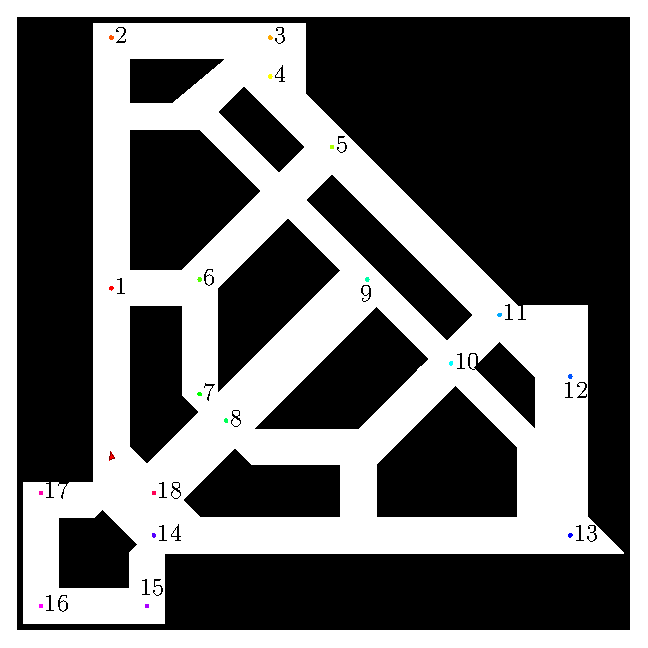
\includegraphics[width=0.33\textwidth]{figs/office}
        \end{figure}
        Office-like Environment
    }
    \only<6>{
        \centering
        \begin{figure}
            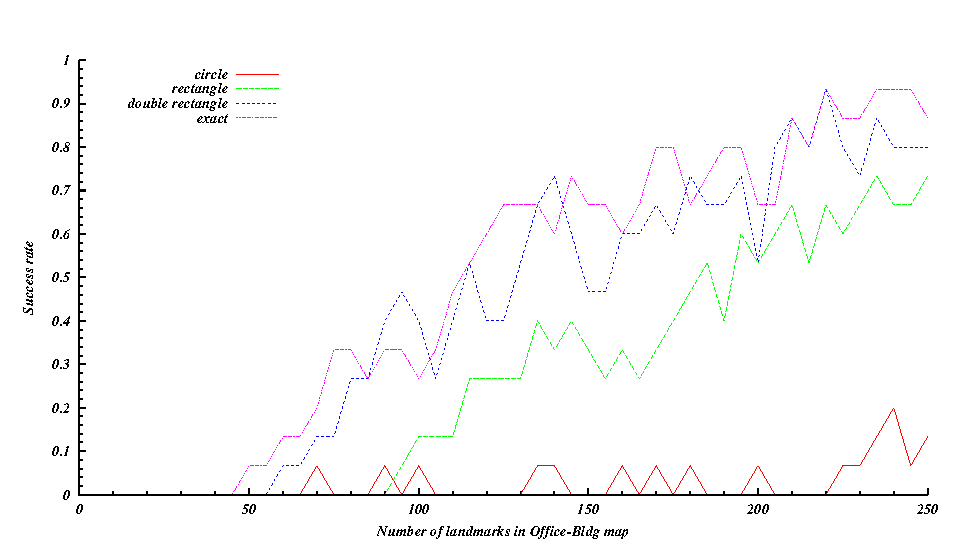
\includegraphics[width=0.67\textwidth]{Data/expnumcse}
        \end{figure}
        Success Rate for the Office-like Environment
    }
\end{frame}